\documentclass[a4paper,10pt,hidelinks]{scrartcl}
%\usepackage[utf8x]{inputenc}

% Packages =========================================
\usepackage{algorithm}
\usepackage{algpseudocode}
\usepackage{amsmath}
\usepackage{amsfonts}   		% Pakete für math. Formeln, Symbole, Ausdrücke
\usepackage{amssymb}
\usepackage[toc,page]{appendix}				% more control over appendices
\usepackage[english]{babel} 				% Anpassung für mehrsprachige Dokumente
\usepackage[usenames, dvipsnames]{color}					% Nutzung von Farben

\usepackage{float}					% notw. für explizite Setzung von Grafiken
\usepackage[T1]{fontenc} 				% Zuweisung Codierschemas für Zeichensätze
\usepackage[paper=a4paper,left=40mm,right=30mm,top=20mm,bottom=25mm]{geometry} % Randmaße
\usepackage{graphicx} 					% Einbindung externer Grafiken
\usepackage{hyperref}
%\usepackage[utf8]{inputenc}				% for german characters like "ä, ö, ü"
%\usepackage{listings}					% notwendig für Quellcode
\usepackage{lmodern}	 				% Moderne Version von Computer Modern
\usepackage{pdfpages}					% Einbindung einer pdf-Datei
\usepackage{pgfplots}
\usepackage{mdwlist}					% kompaktere Auflistungen
\usepackage{microtype}	 				% Optischer Randausgleich
\usepackage[round]{natbib}
\usepackage{doi}
\usepackage{subcaption}					% Subfigure/-tabellen
\usepackage{scrpage2}
\usepackage{tabularx}					% Textsetzung in Tabellen in p-Spalten
\usepackage{textcomp}					% Besondere Textzeichen
\usepackage{ulem}					% Unterstreichung
\usepackage{url}					% Links
\usepackage{xfrac}					% notw. für schräggestellten Bruch
\usepackage[margin=10pt,font=scriptsize,labelfont=bf,labelsep=endash]{caption}




\begin{document}
	\thispagestyle{empty}
	\begin{center}
		\Large
		\textbf{A Neuronal Model for Visually Evoked Startle Responses in Schooling Fish}\\
		
		\vspace*{1cm}
		\normalsize
		Master thesis\\
		
		\vspace{3cm}
		by\\
		Andrej Warkentin \\
		Bernstein Center for Computational Neuroscience - Berlin
		
		\vspace{2cm}
		Supervisors:\\
		Dr. Pawel Romanczuk\\
		Bernstein Center for Computational Neuroscience - Berlin\\
		Prof. Dr. Henning Sprekeler\\
		Technische Universit\"{a}t Berlin
		
	\end{center}
	\pagebreak 
	% Title Page
	\title{masterthesis}
	
	% Inhaltsverzeichnis =====================================
	\thispagestyle{empty}
	\tableofcontents		% Inhaltsverzeichnis erstellen
	\newpage
	%\cleardoublepage	% min. eine Freiseite
	
	%% Für den Hauptteil normale Seitenzahlen
	\pagestyle{useheadings}    % wieder auf normale Seitenrahmen zurück schalten
	\pagenumbering{arabic}  % Nummerierungstyp roman | arabic
	
	\begin{abstract}
		\textbf{Abstract}\\
		Many aspects of fish school behavior can be explained qualitatively by self-propelled agent models with social interaction forces that are based on either metric or topological neighborhoods.
		Recently, startling of fish has been analyzed in its dependence of the network structure \citep{Rosenthal2015} but a mechanistic model and its influence on the collective behavior is missing.
		Here we couple a model for collective behavior with a neuronal model that receives looming visual stimulus input to initiate a startle response, inspired by the neurobiologically well-studied Mauthner cell system.
		First, we analyzed the basic properties of the startle behavior of a single fish as a reaction to a looming stimulus.
		On the group level, we looked at startling frequency as well as group cohesion and polarization depending on neuronal and collective behavior parameters via simulations of the combined model.
		Our results indicate that the startling frequency strongly depends on the dynamics of the group structure, e.g. when the group approaches a boundary of the arena.
		In summary, we took first steps towards a biologically plausible model 
		for startle response initiation in the context of collective motion.
	\end{abstract}
	\newpage
	
	\section{Introduction}
	\begin{itemize}
		\item visual ecology
		\begin{itemize}
			\item warning: making analogies to human vision is almost always misleading
			\item "sensory world of each species is unique"
			\item color vision in fish: Visual Ecology pp. 159
			\item fish orient to overhead polarization orientation in laboratory Hawryshyn 1992
			\item most fish species don't have a fovea (Encyclopedia of Fish 
			Physiology, p. 141) so that eye movements/saccades should not be 
			interpreted as fixations as is the case for humans
			\item they do have different ganglion cell densities though, see 
			\cite{Pita2015}
			\item zebrafish have a row-ordered retinal mosaic with alternating rows with LWS double cones (red and green) and rows with SWS (blue and ultraviolet)
			\item rhodopsin (based on vitamin A1, shorter, "blue" wavelengths) more in marine fish and porphyropsins (based on A2, longer, "green" wavelengths) rather in freshwater fish (more green environment)
			\item important thing to remember: the visual field above a fish is very different from the lateral view which is again different from the visual field below a fish
			\item fritsches and marshall 2002: eye movements in teleosts
			
		\end{itemize}
	\end{itemize}
	\section{Methods and Materials}
	\begin{itemize}
		\item first paragraph
	\end{itemize}
	\section{Results}
	\subsection{Response properties of a single LIF neuron}
	As a first step we presented a single LIF neuron with the visual angle 
	$\theta$ over time as input current.
	In order to compare our results with experimental work (see e.g. 
	\cite{Bhattacharyya2017}, \cite{Temizer2015}, \cite{Dunn2016}) we analyzed 
	the angle, distance, latency and time-to-collision of the response.
	The response onset was defined as the time of the first spike of the LIF neuron.
	We ignore further processing time after the spike of the Mauthner cell 
	because it is in the order of milliseconds (\cite{Preuss2003}) and thus 
	irrelevant with respect to the overall response time which is in the order 
	of at least hundreds of milliseconds for visual stimuli 
	\citep{Preuss2006}.\\
	In the model, we used the basic electrophysiological parameters that were measured in larval zebrafish 4 days post-fertilization \citep{Koyama2016} and kept them fixed for all simulations.
	We analyzed the effects of parameters of a linear transformation of the input, i.e. the slope and offset and furthermore the effects of noise on the input, on the initial condition, and on the spiking threshold.
	%TODO: add variable names
	%TODO: add formulas
	All parameters are listed in table \ref{tab:params}.\\
	effects:
	\begin{itemize}
		\item effects of increasing m:
		\begin{itemize}
			\item mean response distance: mean increases linearly independent 
			of threshold noise (only for high threshold noise slightly 
			sub-linear)
			\item variance of response distance: increases linearly for small 
			threshold noise (except for a high lv value and low threshold 
			noise, this is due to a very low mean and outliers that distort the 
			standard deviation estimate), increases sub-linearly for medium 
			threshold noise, slightly decreases for high threshold noise
			\item mean response angle: decreases exponentially  independent of 
			threshold noise
			\item variance of response angle: slightly decreases independent of 
			threshold noise
			\item mean time to collision: absolute value increases linearly 
			independent of threshold noise, decreases more strongly for higher 
			L/V values
			\item variance of time to collision: very small increases for L/V 
			values smaller than 0.9, for L/V values above 0.9 the variance is 
			in general higher, for small threshold noise it is smallest for 
			medium m-values and for higher threshold noise it also increases 
			with m
			\item mean response time: very similar to TTC
		\end{itemize}
		\item effects of increasing threshold noise:
		\begin{itemize}
			\item mean response distance: 
		\end{itemize}
	\end{itemize}
	\begin{table} [!th]
		\begin{center}
			\begin{tabular}{|l|c|p{7cm}|}
				\hline
				\textbf{Parameter} & \textbf{Value (unit)} & \textbf{Comment} \\
				\hline
				$E_L$ & -79 mV & Resting potential\\
				$R_M$ & 10 MOhm & Membrane resistance\\
				$\tau_{m}$ & 23 ms & Membrane time constant\\
				$V_t$ & -61 mV & Mean spiking threshold\\
				$dt$ & 0.001 s & Integration time step\\
				$T$ & 5 s & Total time\\
				$sd_{thr}$ & 1 mV & Standard deviation of spiking threshold noise\\
				$sd_{I}$ & 5 mV & Standard deviation of input noise\\
				$sd_{init}$ & 1 mV & Standard deviation of initial condition noise\\
				$m$ & 1 \textdegree/s  & Slope of linear transformation\\
				$b$ & 0 \textdegree & Offset of linear transformation\\
				\hline
			\end{tabular}
		\end{center}
		\caption{Parameters of the single LIF neuron model with a looming stimulus input. Parameters that were explored are indicated either by a value range such as e.g. for $\mu_s$ or by a set with all explored values inside of curly brackets such as e.g. for $\sigma_s$.}
		\label{tab:params}
	\end{table}
	\begin{itemize}
		\item Effect of input transformation
		\item Effect of different noise sources
		\item Effect of input type
	\end{itemize}
	\subsection{Input}
	\begin{itemize}
		\item 
	\end{itemize}
	\subsection{Feedforward inhibition}
	\begin{figure}[H]
		\centering
		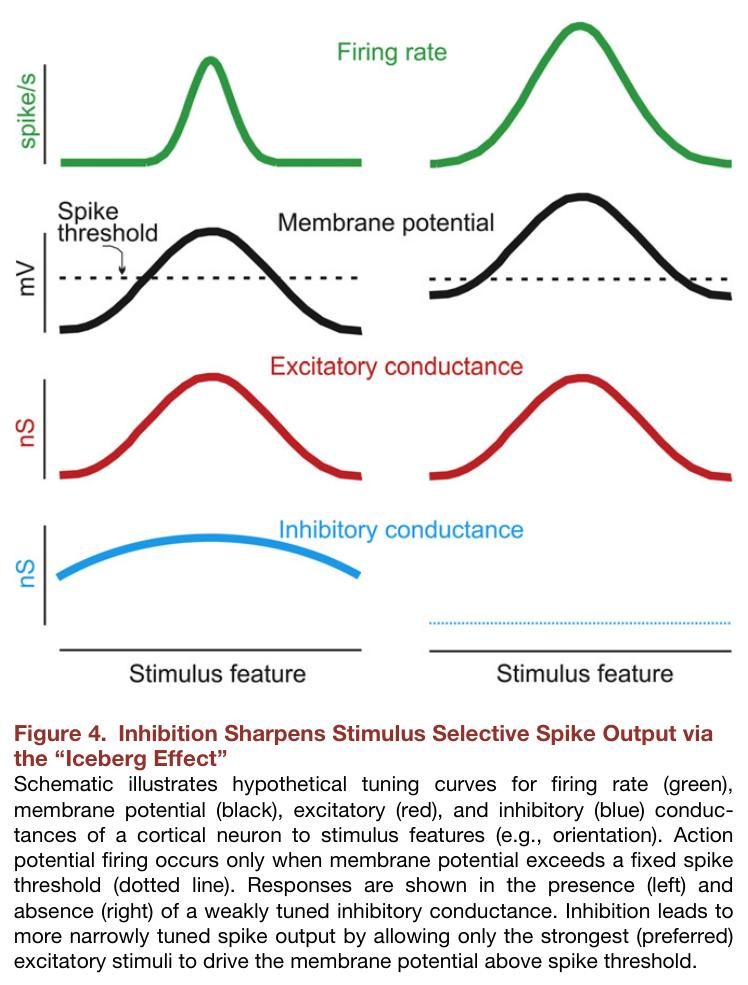
\includegraphics[width=0.6\textwidth, 
		height=0.4\textheight]{../figures/isaacson2001_figure4.jpg}
		\caption{how input sharpens tuning. From \cite{Isaacson2011}}
		\label{fig:feedf}
	\end{figure}
	\begin{itemize}
		\item 
	\end{itemize}
	\subsection{Cross-inhibition}
	\begin{itemize}
		\item 
	\end{itemize}
	\subsection{Feedback inhibition}
	\begin{itemize}
		\item 
	\end{itemize}
	\section{Discussion}
	\begin{itemize}
		\item we focus here on the experimental results from 
		\cite{Bhattacharyya2017} but one should keep in mind that their results 
		might be specific to properties of experiment such as fish handling, 
		fish age, species, arena, environment, stimulus setup (projection on 
		screen)
	\end{itemize}
	\newpage
	\bibliographystyle{abbrvnat}
	\bibliography{masterthesisbib}
	
	\newpage
	\appendix
	%\appendixheaderon
		% next line tells latex to not list sections in the Table of Contents, \protect is needed because \setcounter apparantly
		% is a fragile command (see http://www.tex.ac.uk/FAQ-protect.html)
	\addtocontents{toc}{\protect\setcounter{tocdepth}{-1}}
	\section{Appendix}

	
\end{document}          
